% Exercise Template
%A LaTeX template for typesetting exercise in Persian (with cover page).
%By: Reza Adinepour

\documentclass[12pt]{exam}

\usepackage{setspace}
\usepackage{listings}
\usepackage{graphicx,subfigure,wrapfig}
\usepackage{multirow}
\usepackage{matlab-prettifier}
\usepackage{amsmath}
\usepackage{multicol}


\usepackage[margin=20mm]{geometry}
\usepackage{xepersian}
\settextfont{XB Niloofar}

\newcommand{\class}{آزمایشگاه DSP}
\newcommand{\term}{نیم‌سال دوم ۰۱-۰۲}
\newcommand{\college}{دانشکده مهندسی برق}
\newcommand{\prof}{استاد: دکتر مقیمی}

\singlespacing
\parindent 0ex

\begin{document}


% -------------------------------------------------------
%  Thesis Information
% -------------------------------------------------------

\newcommand{\ThesisType}
{سمینار}  % پایان‌نامه / رساله
\newcommand{\ThesisDegree}
{کارشناسی ارشد گرایش معماری کامپیوتر}  % کارشناسی / کارشناسی ارشد / دکتری
\newcommand{\ThesisMajor}
{مهندسی برق}  % مهندسی کامپیوتر
\newcommand{\ThesisTitle}
{ساعت دیجیتال}
\newcommand{\ThesisAuthor}
{رضا آدینه پور-9814303\\علی‌رضا قربانی-9823263}
\newcommand{\ThesisSupervisor}
{جناب آقای دکتر رضا خرقانیان}
\newcommand{\ThesisDate}
{خرداد 1402}
\newcommand{\ThesisDepartment}
{دانشکده مهندسی برق}
\newcommand{\ThesisUniversity}
{دانشگاه صنعتی شاهرود}

% -------------------------------------------------------
%  English Information
% -------------------------------------------------------

\newcommand{\EnglishThesisTitle}{A Standard Template for Course Exercise}


\pagestyle{empty}
\include{cover-page}

% These commands set up the running header on the top of the exam pages
\pagestyle{head}
\firstpageheader{}{}{}
\runningheader{صفحه \thepage\ از \numpages}{}{\class}
\runningheadrule

\vspace{0pt}




\begin{questions}
\pointpoints{نمره}{نمره}

\question
بدون استفاده از توابع آماده متلب، تابعی بنویسید که یک سیگنال و عددی بعنوان طول فیلتر میانگین متحرک «\lr{Moving average}» از کاربر بگیرد و نتیجه اعمال فیلتر مذکور بر روی سیگنال را نشان دهد. « واضح است که طول فیلتر باید عددی فرد باشد. بنابراین انتظار می‌رود برنامه به گونه‌ای نوشته شود که اعداد فرد را بعنوان طول فیلتر از کاربر بگیرد. همچنین برای اعمال فیلتر به نقاط ابتدایی و انتهایی سیگنال از تکنیک افزودن صفر «\lr{Zero Padding}» استفاده کنید. \\

• تابع نوشته شده به‌صورت زیر است: 
\begin{latin}
\begin{lstlisting}[
	frame=single,
	numbers=left,
	style=Matlab-editor %style: % Matlab-editor, Matlab-Pyglike, Matlab-bw
	] 
	
function filtered_signal = moving_average_filter(input_signal, filter_length)
	% input_signal: vector of the input signal
	% filter_length: odd number for length of the moving average filter
	
	if (mod(filter_length, 2) == 0)
		warning('Filter length should be odd. Rounding up to nearest odd number.');
		filter_length = filter_length + 1;
	end
	
	% Pad input signal with zeros at the beginning and end to ensure that the
	% output signal is the same length as the input signal
	pad_length = floor(filter_length / 2);
	padded_signal = [zeros(pad_length, 1);
	input_signal;
	zeros(pad_length, 1)];
	
	% Initialize output signal
	filtered_signal = zeros(size(input_signal));
	
	% Calculate the moving average for each element in the input signal
	for i = 1:length(input_signal)
		filtered_signal(i) = mean(padded_signal(i:i + filter_length - 1));
	end
end

\end{lstlisting}
\end{latin}

\question
به‌منظور برسی کارایی تابع نوشته شده،‌یک سیگنال سینوسی بسازید و مقدار کم و مناسبی نویز «می‌توانید از تابع نوشته شده در تمرین قبل استفاده نمایید» با استفاده از تابع rand متلب به آن اضافه کنید و کارایی فیلتر میانگین متحرک به منظور کاهش نویز را برای طول‌های مختلف 3، 5، 7، 9 امتحان کنید. \\
\\

• کد نوشته شده برای تست تابع به‌صورت زیر است: 
\begin{latin}
	\begin{lstlisting}[
		frame=single,
		numbers=left,
		style=Matlab-editor %style: %Matlab-Pyglike, Matlab-bw
		] 
clear; clc; close all;

% Generate a sample input signal
Fs = 1e3;
t = 0:1/Fs:1;
f = 5;
x = sin(2 * pi * f * t);
SNR = input('Enter the desired SNR value: ');
noisy_signal = add_noise(x, SNR);

% Calculate the legth of moving average filter
filter_length = input('Enter length of filter(must be odd): '); % [3, 5, 7, 9]

figure(1);
subplot(length(filter_length)+1, 2, 1);
plot(t, x);
title('input signal without noise');
xlabel('time');
ylabel('amplitude')
grid on;
grid minor;

subplot(length(filter_length)+1, 2, 2);
plot(t, noisy_signal);
title(['noisy signal with SNR = ', num2str(SNR), 'dB']);
xlabel('time');
ylabel('amplitude')
grid on;
grid minor;

for j=1:length(filter_length)
	filtered_signal = moving_average_filter(noisy_signal', filter_length(j));
	subplot(length(filter_length)+1, 2, j + 2);
	plot(t, filtered_signal);
	title(['filtered signal with N = ', num2str(filter_length(j))]);
	xlabel('time');
	ylabel('amplitude')
	grid on;
	grid minor;
end
		
\end{lstlisting}
\end{latin}

• خروجی برنامه به‌صورت زیر است: 
\begin{figure}[t]
	\centering
	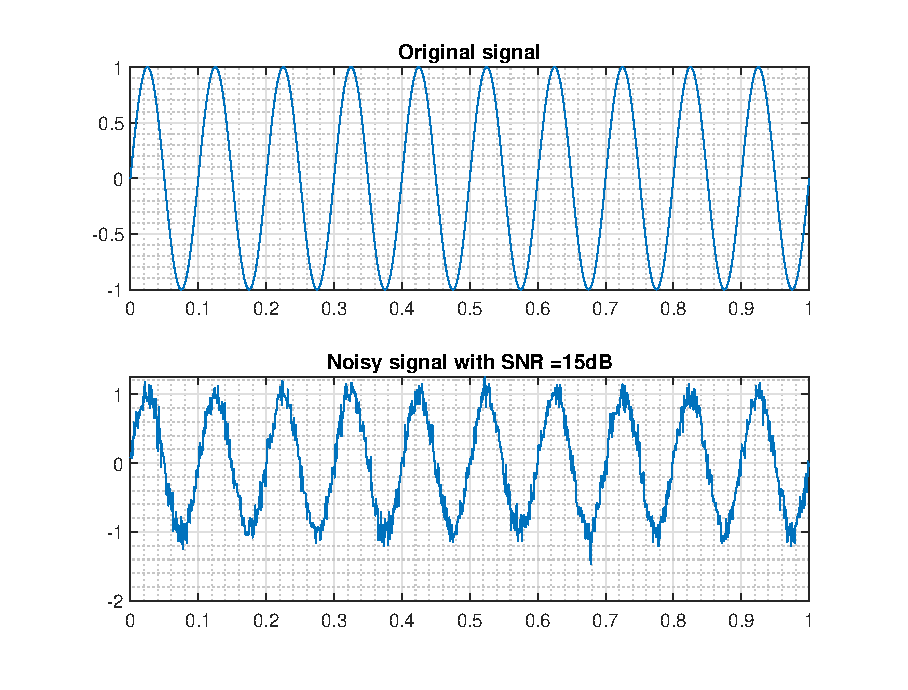
\includegraphics[width=1\textwidth]{images/Result}
	\caption{خروجی برنامه}
\end{figure}


\end{questions}
\end{document}

